\clearpage
\section{Realisierung Gehäuse}\label{sec:Realisierung Gehäuse}
Im folgenden Teil des Fachberichtes ist die Realisierung des Gehäuse beschrieben. 

Die Anforderungen an das Gehäuse des digitalen Theremin sind:
\begin{itemize}
	\item Die Volume und die Pitch Antenne müssen genügend Abstand zueinander haben.
	\item Das Antennenoszillator PCB und das DE1-SoC Board müssen für den Spieler ersichtlich sein.
	\item Für die Bedienung muss das LT24 Touch Module für den Benutzer gut sichtbar platziert sein.
	\item Um den Preis des Gehäuses tief zu halten und für die Gestaltung des Gehäuses möglichst viel Freiheit zu haben, wird das Gehäuse 3D-gedruckt.  
\end{itemize}

Um diese Anforderungen zu erfüllen entschiedenen wir uns das Gehäuse mit dem 3D-CAD-System Inventor zu konstruieren. Inventor ist eine sehr umfangreiche Konstruktion Software die einige nützliche Funktionen enthält um 3D Modelle zu erstellen. Zudem können Studenten für ein Jahr lang die Software für nicht kommerzielle Zwecke frei nutzen\cite{Inventor}.
Um das Gehäuse zu drucken hatten wir uns entschieden den S5 Ultimaker 3D Drucker zu verwenden, da dieser sehr benutzerfreundlich ist und ein grosses Druckvolumen hat. 
Der S5 Drucker hat eine Druckvolumen von \SI{330x240x300}{mm}. 
Im Verlauf der Realisierung des Gehäuses stellte sich jedoch heraus das, dass Gehäuse bedeuten grösser wird als das Druckvolumen des Druckers. Da wir kein 3D Drucker mit grösserem Druckvolumen zur Verfügung hatten, ist das Gehäuse in vier Einzelteilen konstruiert. 

Wir entschieden uns die Form des Theremin oval zu gestalten, da der 3D-Drucker diese Geometrie erlaubt. Die vier Einzelteile des Gehäuses sind alle gleich aufgebaut. Abbildung \ref{img:grundteil} zeigt die Grundstruktur eines Einzelteil. Die Funktion Wandung ermöglichte es die Grundstruktur oval auszuhöhlen. Jeweils zwei Einzelteile bilden zusammen den Deckel und den Boden. Daraus resultierte das in Abbildung \ref{img:Theremin_case} gezeigte Gehäuse. 

Die vier Einzelteile sind aus schwarzem Polylactide (PLA)  gedruckt. Da das Gehäuse eine ovale Geometrie hat, braucht es Stützstrukturen für den Herstellungsprozess. Das eingesetzte Polyvinylalkohol (PVAL) hat die nützliche Eigenschaft das es  wasserlössliche ist. Nachdem das Bauteil einigen Stunden im Wasser eingelegt war, verschwanden die Stützstrukturen sehr gründlich. 
Das drucken der vier Einzelteilen dauerte insgesamt sechs Tage.
\begin{figure}[h]
	\centering
	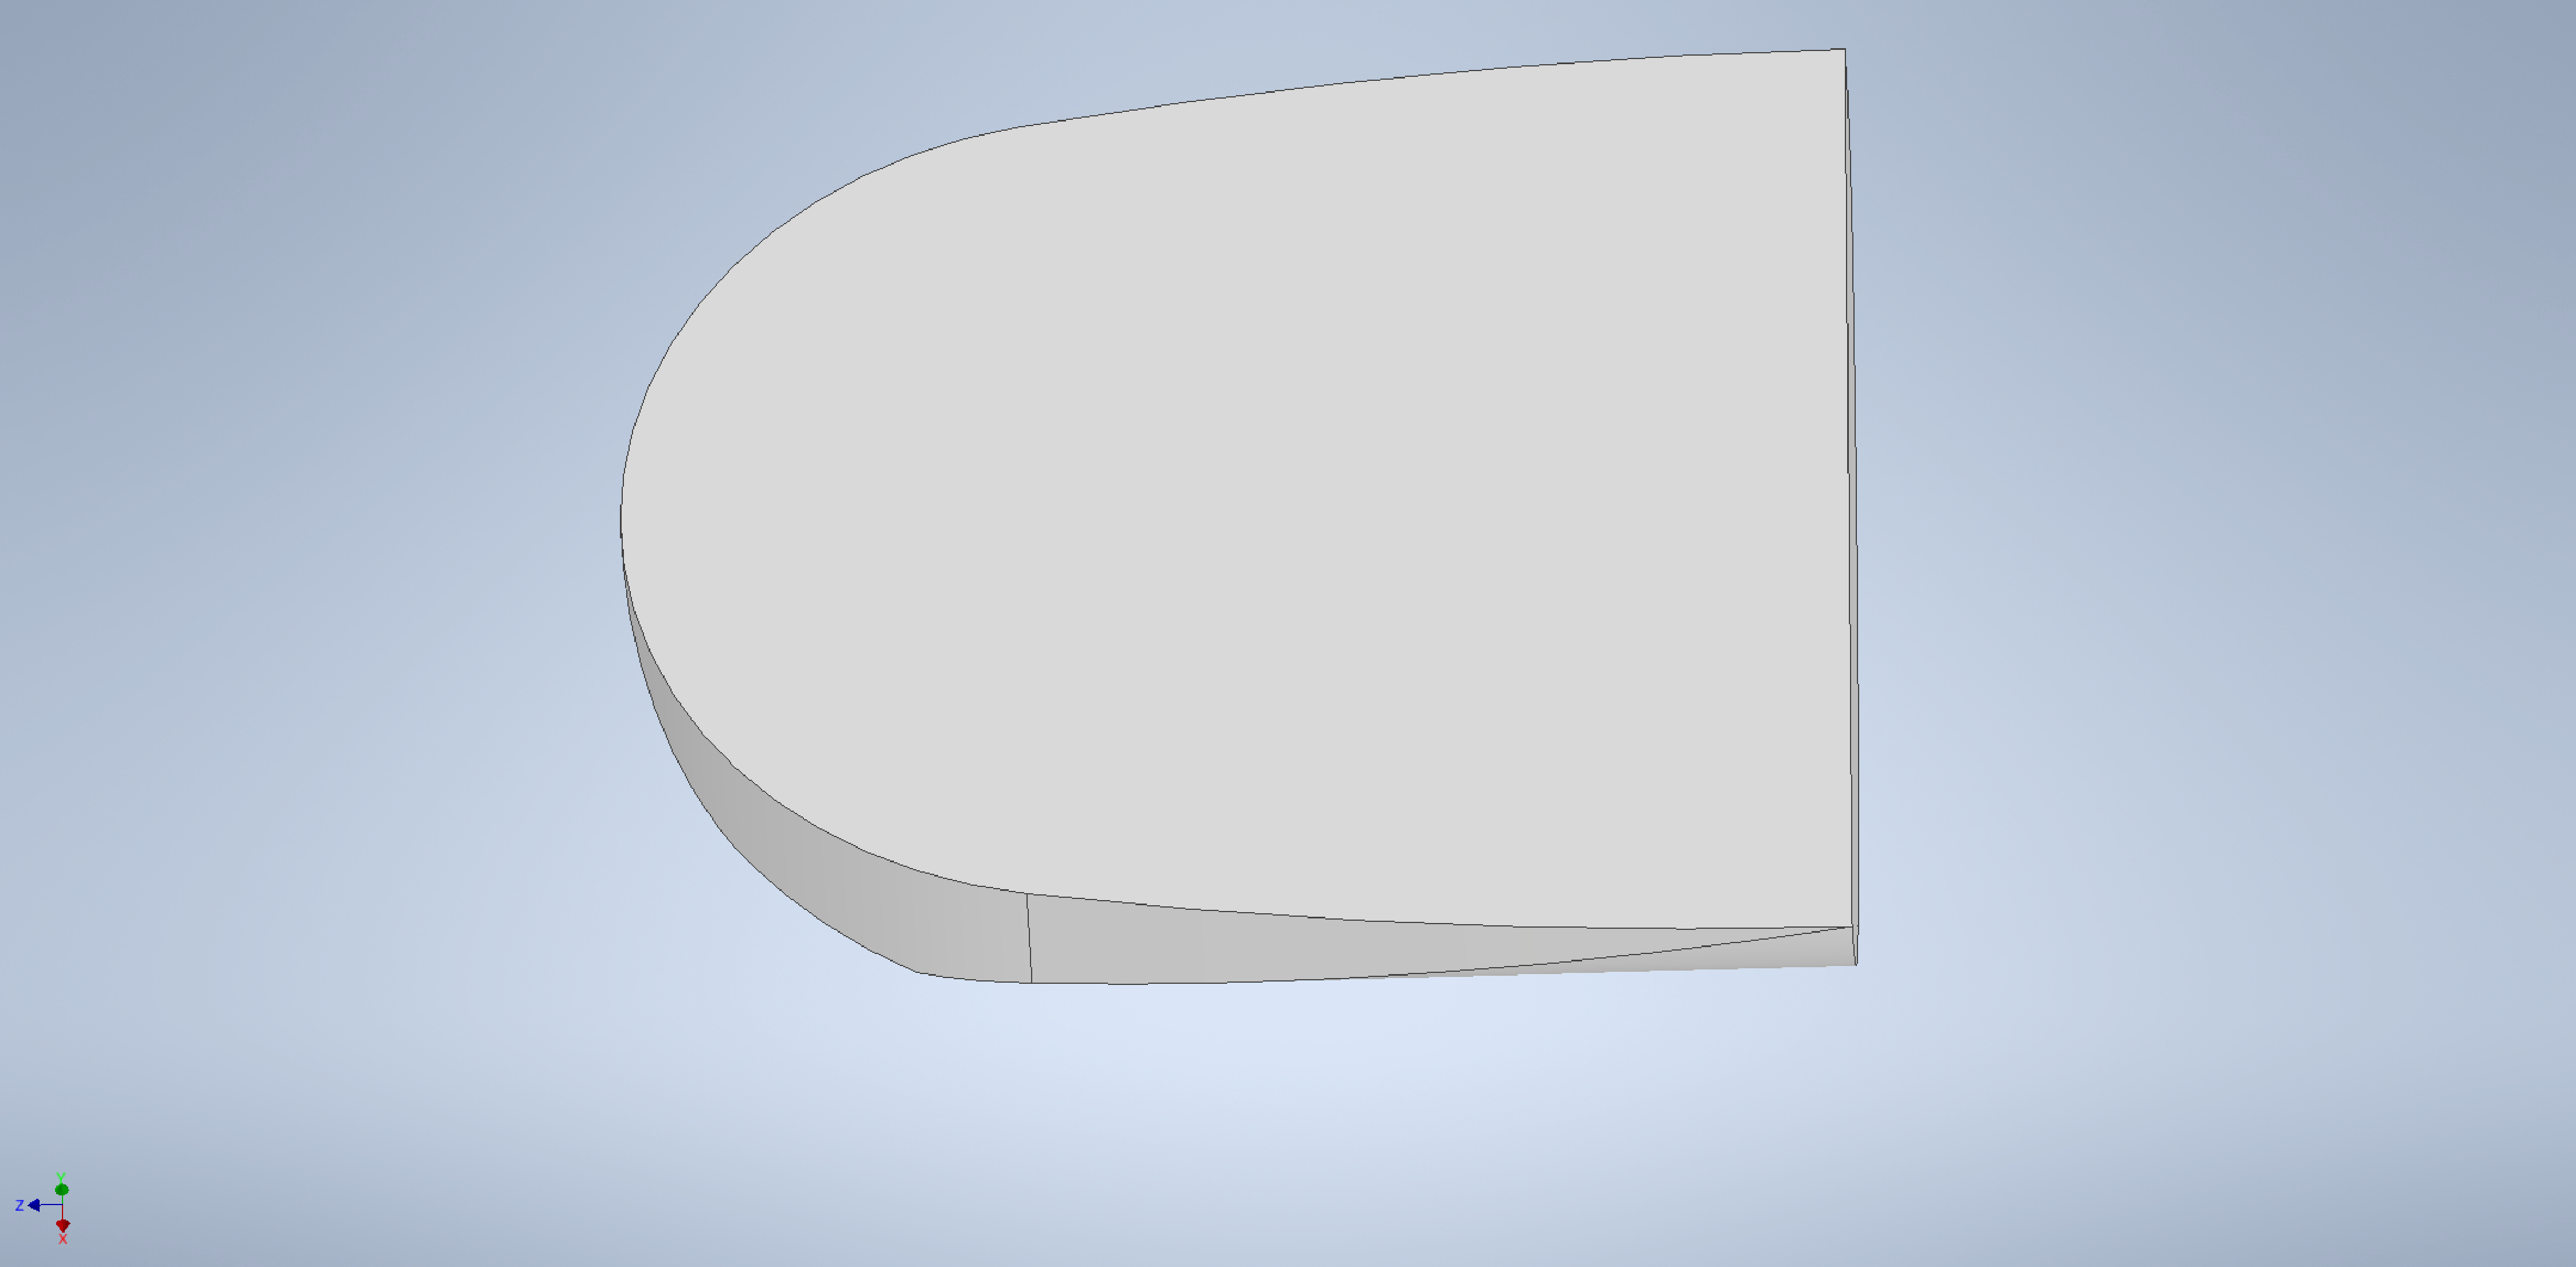
\includegraphics[width=\textwidth]{grundteil.pdf}
	\caption{Grundstruktur eines Einzelteils.}
	\label{img:grundteil}
\end{figure}
\begin{figure}[h]
	\centering
	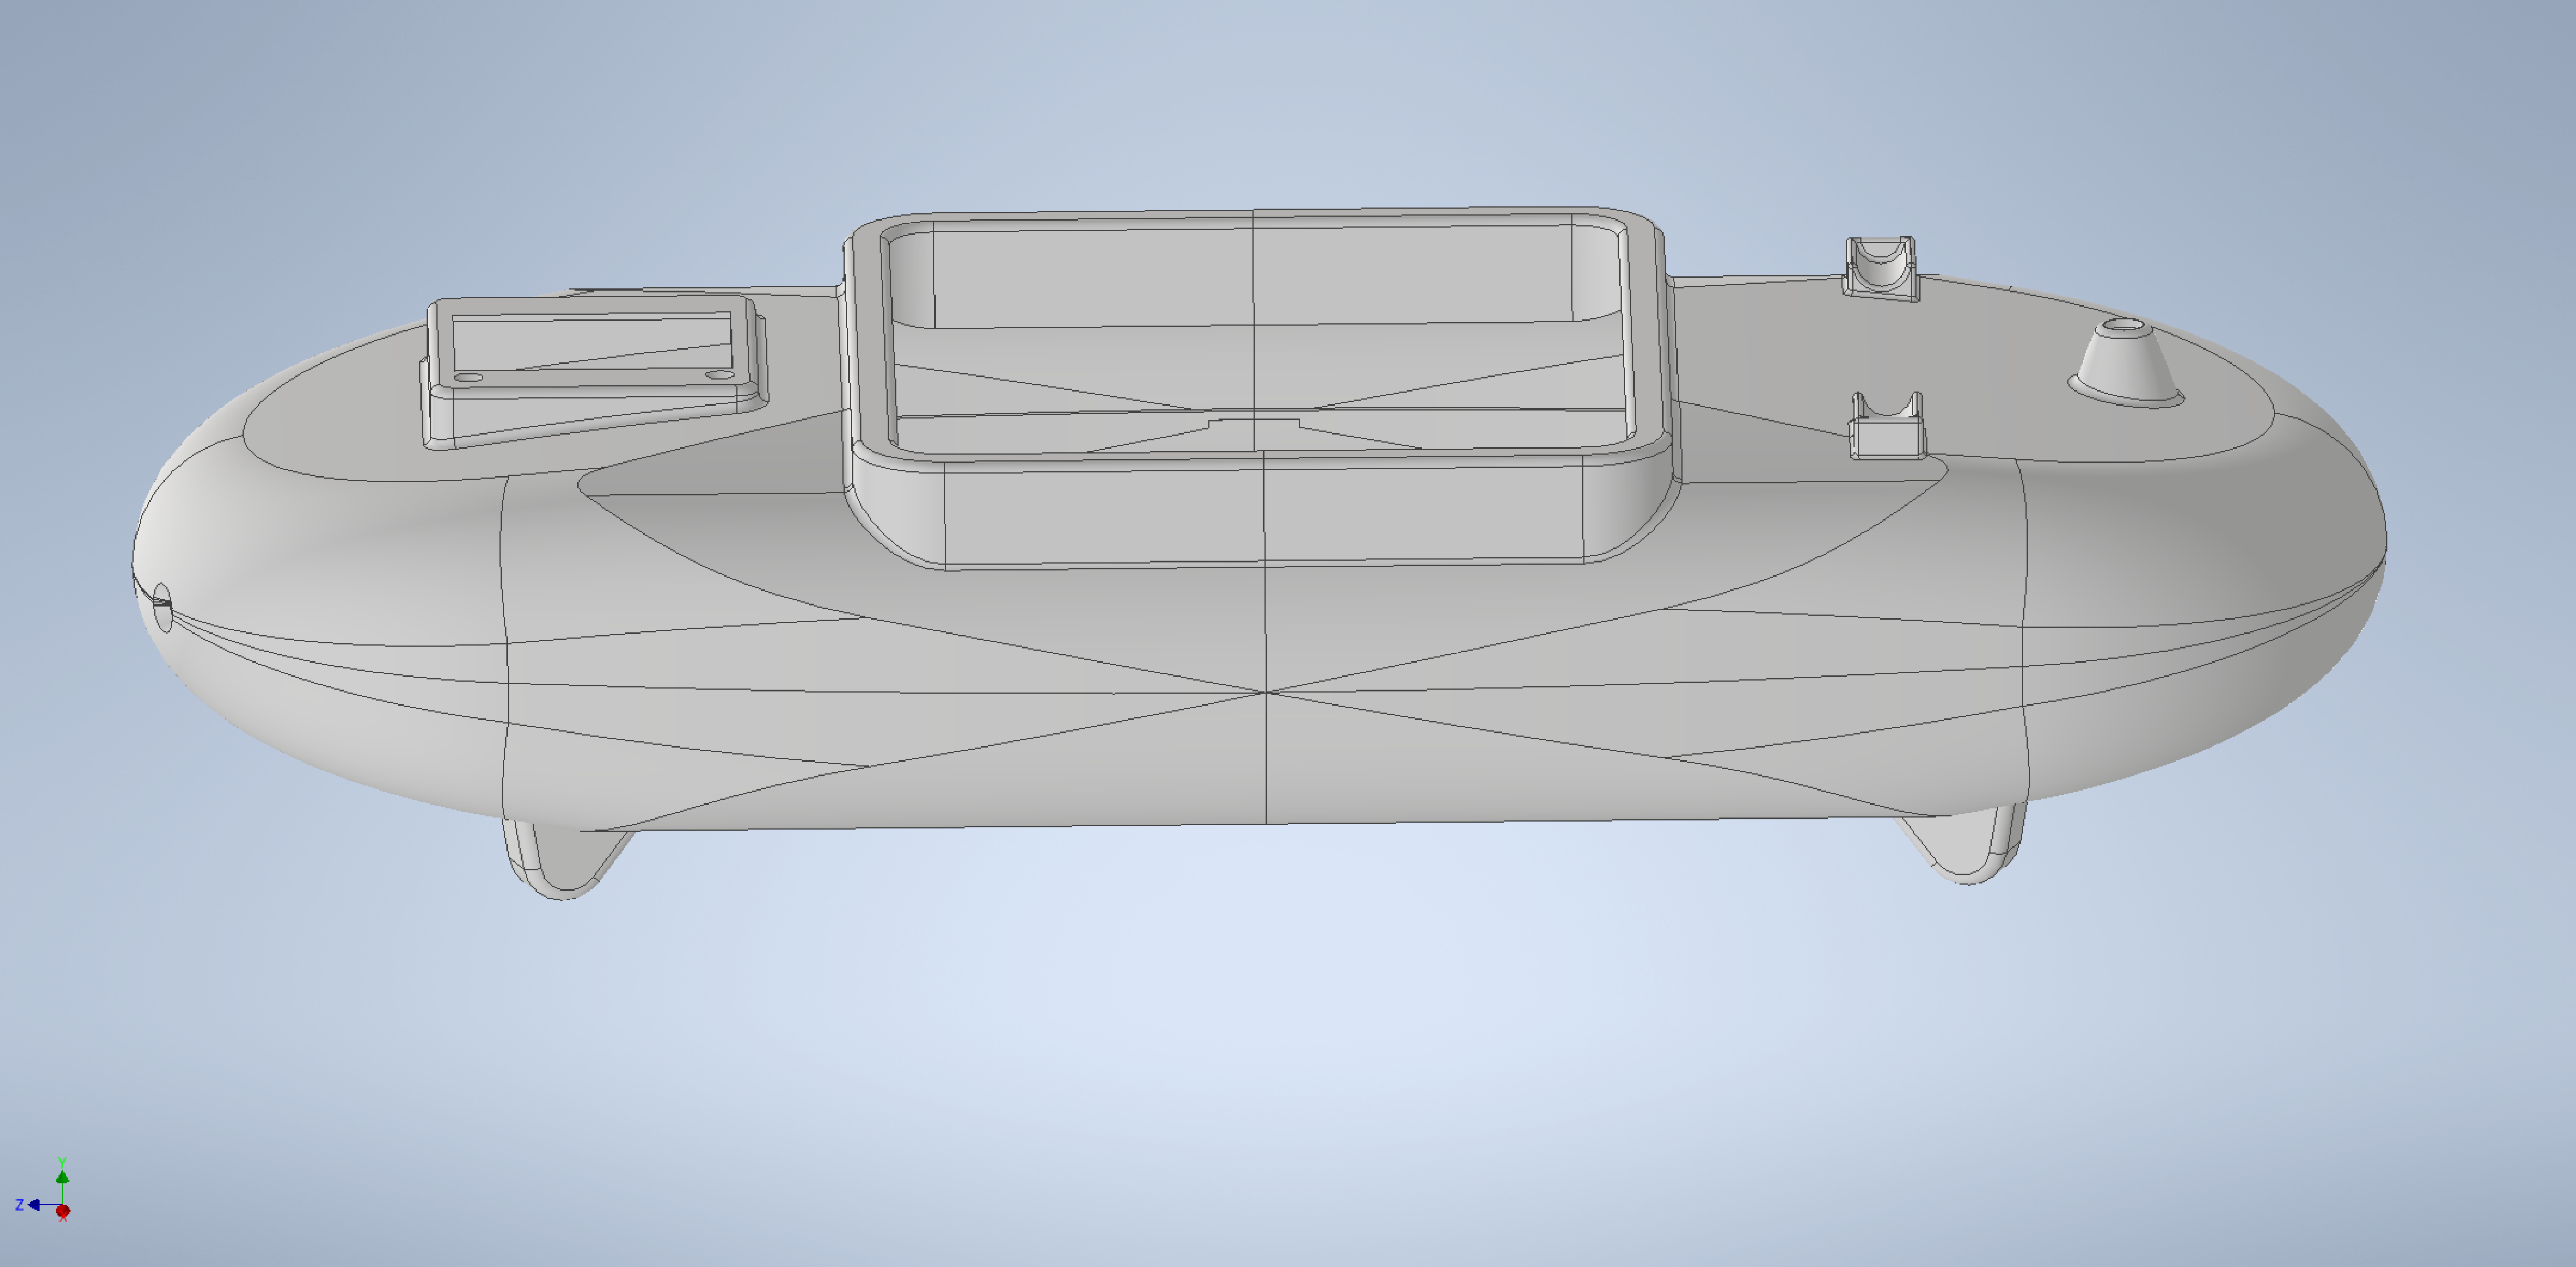
\includegraphics[width=\textwidth]{Theremin_case.pdf}
	\caption{Theremin Gehäuse.}
	\label{img:Theremin_case}
\end{figure}




